\documentclass[conference]{IEEEtran}
\IEEEoverridecommandlockouts
% The preceding line is only needed to identify funding in the first footnote. If that is unneeded, please comment it out.
\usepackage{cite}
\usepackage{amsmath,amssymb,amsfonts}
\usepackage{algorithmic}
\usepackage{graphicx}
\usepackage{textcomp}
\usepackage{xcolor}
\usepackage{booktabs}
\usepackage{subcaption}
\usepackage{multirow}
\usepackage{svg}
\usepackage{hyperref}

\DeclareMathOperator*{\argmax}{arg\,max}
\def\eg{\emph{e.g. }}
\def\Eg{\emph{E.g.}}
\def\etal{\emph{et al. }}
\def\ie{\emph{i.e. }}
\def\Ie{\emph{I.e. }}


\def\BibTeX{{\rm B\kern-.05em{\sc i\kern-.025em b}\kern-.08em
    T\kern-.1667em\lower.7ex\hbox{E}\kern-.125emX}}
\begin{document}

\title{Towards Clear Evaluation of Robotic Visual Semantic Navigation \\
\thanks{This research was funded by projects: AIRPLANE, with reference PID2019-104323RB-C31; EYEOT, with reference PID2021-128362OB-100; and POLLUTWIN, with reference TED2021-129162B-C22 from the Ministry of Science and Innovation of Spain.}
}

% \author{\IEEEauthorblockN{1\textsuperscript{st} Given Name Surname}
% \IEEEauthorblockA{\textit{dept. name of organization (of Aff.)} \\
% \textit{name of organization (of Aff.)}\\
% City, Country \\
% email address}
% \and
% \IEEEauthorblockN{2\textsuperscript{nd} Given Name Surname}
% \IEEEauthorblockA{\textit{dept. name of organization (of Aff.)} \\
% \textit{name of organization (of Aff.)}\\
% City, Country \\
% email address}
% \and
% \IEEEauthorblockN{3\textsuperscript{rd} Given Name Surname}
% \IEEEauthorblockA{\textit{dept. name of organization (of Aff.)} \\
% \textit{name of organization (of Aff.)}\\
% City, Country \\
% email address}
% }

\author{
\IEEEauthorblockN{
Carlos Guti\' errez-\'Alvarez\IEEEauthorrefmark{1}, Sergio Hern\'andez-Garc\'ia\IEEEauthorrefmark{2}, Nadia Nasri\IEEEauthorrefmark{1}\IEEEauthorrefmark{3}, \\ Alfredo Cuesta-Infante\IEEEauthorrefmark{2} and Roberto J. L\'opez-Sastre\IEEEauthorrefmark{1}}
\IEEEauthorblockA{\IEEEauthorrefmark{1}University of Alcal\'a, Department of Signal Theory and Communications, Alcal\'a de Henares, Spain\\
Email: \{carlos.gutierrezalva, nadia.nasri, robertoj.lopez\}@uah.es}
 \IEEEauthorblockA{\IEEEauthorrefmark{2}Rey Juan Carlos University, Superior Polytechnic School of Computer Science, M\'ostoles, Spain\\
Email: \{sergio.hernandez, alfredo.cuesta\}@urjc.es}
\IEEEauthorblockA{\IEEEauthorrefmark{3}University of Alicante, Institute for Computer Research, Alicante, Spain}
}


\maketitle

\begin{abstract}
In this paper we address the problem of visual semantic navigation (VSN), in which a robot needs to navigate through an environment to reach an object having only access to egocentric RGB perception sensors.
This is a recently explored problem, where most of the approaches leverage last advances in deep learning models for visual perception, combined with reinforcement learning (RL) strategies.
Nonetheless, after a review of the literature, it is complicated to perform direct comparisons between the different solutions.
The main difficulties lie in the fact that the navigation environments in which the experimental metrics are reported are not accessible, and each approach uses different RL libraries.
In this paper, we release a publicly available experimental setup for the VSN problem, with the aim of providing a clear benchmark.
It has been constructed using pyRIL, an open source python library for RL, and two navigation environments: Miniwolrd-Maze from gym-miniworld, and one 3D scene from HM3D dataset using AI Habitat simulator.
We finally propose a state-of-the-art VSN model, consisting in a Contrastive Language Image Pretraining (CLIP) visual encoder plus a set of two recurrent neural networks for producing the discrete navigation actions.
This model is evaluated in the proposed experimental setup, with a careful analysis of the main VSN challenges, namely: the sparse rewards problem; and the exploitation-exploration trade-off.
Code is available at: \url{https://github.com/gramuah/vsn}.
\end{abstract}

\begin{IEEEkeywords}
navigation, reinforcement learning, robot, deep learning
\end{IEEEkeywords}

\chapter{Introduction}\label{ch:introduction}

\setlength\epigraphwidth{.69\textwidth}
\epigraph{\itshape ---The most important step a man can take.
It's not the first one, is it?
---It's the next one.
Always the next step, Dalinar.}{Brandon Sanderson, \textit{Oathbringer.}}

\lettrine{\textcolor{accent_color}{W}}{ho} has never dreamt of a robot friend?
A robot that can help you with your daily tasks, play games with you, help you with your homework, or even be your personal assistant?
The idea of having a robotic companion is not new, for it has remained a dream for humanity for a long time.
Since the first mention of the term \textit{robot}~\cite{robot1920}, this aspiration has been only possible in science fiction movies and books.
However, with the recent advancements in robotics and \acrfull{ai}, humanity is closer than ever to this reality.
This humble thesis is nothing more than just a small step towards the joint effort of achieving this dream.

Now, how do we create a robot that can be a friend to humans?
This simple question omits a multitude of challenges that need to be addressed.
Some of these challenges include the robot's ability to understand and interact with humans, its ability to learn from its environment, or its ability to adapt to different situations.
However, there is one aspect underlying all these challenges; \textit{movement}:

\begin{itemize}
    \item A robot that understands and interacts with humans \textit{must be able to move} in order to follow the humans and interact with them.
    \item A robot that learns from its environment \textit{must be able to move} in order to explore and gather information.
    \item A robot that adapts to different situations \textit{must be able to move} in order to change its behavior and actions based on the environment.
\end{itemize}

Moreover, it has been thoroughly discussed in the literature that movement is a fundamental aspect of intelligence~\cite{Darwin1871, Arbib2005, Leisman2016, Wolpert2011, Llinas2001}.
This clearly shows that movement is a crucial component of any intelligent system known to us.
If we want to create any intelligent entity that somehow resembles our own intelligence, we must first address the problem of movement.

This thesis is dedicated to the study of movement in robots, specifically in the context of embodied \acrshort{ai}.
This topic is known as \acrfull{vsn}, in which an agent must navigate in an environment to accomplish certain tasks while only relying on visual information.
On \acrshort{vsn} there is no prior knowledge of the environment or any map that the agent can consult.
The agent must learn to navigate in the environment by exploring it and learning from its own experiences.
It has to understand the scene not only geometrically, but also semantically.
If not, it will not be able to understand the meaning of the objects in the scene and how they relate to each other.
For example, if the agent is placed in a bedroom and asked to find a fridge, it must understand that the fridge is not (typically) in the bedroom and that it must navigate to the kitchen to find it.

\acrshort{vsn} tasks are very challenging, and as one may expect, they typically need a careful design of a complex system that combines multiple components in charge of different aspects of the navigation.
Many works~\cite{newcombe2011, thrun2001, jones2011, sattler2018, Kazerouni2022, campos2021, labbe2022, zhang2018, rosinol2020, jin2023} follow this approach, and they typically rely on a combination of visual perception, semantic understanding, and navigation planning.
However, \acrshort{vsn} can be also formulated as a \acrfull{rl}~\cite{sutton2018} problem.
\acrshort{rl} is a whole artificial intelligent framework that allows an agent to learn how to act in an environment by receiving rewards for its actions.
The rewards are typically defined in terms of the agent's performance in the task, such as reaching a goal or avoiding obstacles.
By following an iterative process within the environment, the agent can learn how to maximize its rewards and complete its tasks.

The main goal of this thesis is to study the \acrshort{rl} and \acrshort{vsn} powerful combination that allows agents to be trained to navigate in an environment.
After intensive training, agents can learn to navigate by trial and error, obtaining rewards that guide them to the goal.
In figure~\ref{fig:abstract_thesis}, an abstract representation of the thesis's framework is shown.
In it, an agent, by interacting with the environment, learns to navigate to a goal.
In the environment, even though there is not a map present, the agent can learn to understand the scene and the objects in it.
By these semantic cues, the agent can learn to navigate to the goal, even if it is not visible in the scene.

\begin{figure}
    \centering
    \includegraphics[trim=30 30 30 30, clip, width=\textwidth]{figures/introduction/abstract_thesis}
    \caption[The framework of \acrshort{rl} and \acrshort{vsn}]{\textbf{The framework of \acrshort{rl} and \acrshort{vsn}}.
    Navigating in an environment is a complex task that requires the agent to learn how to interact with the environment and understand the scene.
    The agent learns to navigate by trial and error, obtaining rewards that guide it to the goal. In this way, the agent can learn to understand the scene and the objects in it, even if there is no prior knowledge of the environment or any map that it can consult.}
    \label{fig:abstract_thesis}
\end{figure}

\section{Motivation}\label{sec:motivation}

This thesis is part of the AIRPLANE (\acrshort{ai} and Robotic Mobile PLAtforms to Improve Disabled People INdependencE) research project conducted in the~\href{https://gramweb.uah.es/}{GRAM research group} of the~\href{https://www.uah.es/en/}{University of Alcalá}.
The AIRPLANE project focuses primarily on creating new mobile robotic platforms that incorporate advanced perception, interaction, and navigation capabilities to enhance the independence of people with functional diversity.
The main goal in the AIRPLANE project is to build a low-cost mobile platform that integrates the latest advances in \acrshort{ai} and computer vision.
Specifically, it will equip the platform with the ability to navigate real environments and develop online action-recognition solutions that enable interaction applications for users with functional diversity.
And, as shown in the figure~\ref{fig:icra_papers}, the interest in this topic is not only limited to the AIRPLANE project, but it is also a hot topic in the robotics community.
Therefore, the first step is to study \acrshort{vsn} solutions that allow the robot to navigate using \acrshort{rl} algorithms.

The \acrshort{vsn} problem is very broad, and it can be applied to many different scenarios.
For example, it can be used to navigate in indoor environments, such as homes or offices, or in outdoor environments, such as streets or parks.
It can be used to navigate in environments with different types of obstacles, such as furniture or people, or in environments with different types of goals, such as finding a specific object or reaching a specific location.
It can also be used to perform different types of tasks, such as rearranging objects~\cite{NEURIPS2021_021bbc7e}, navigating to them~\cite{batra2020}, or even performing a natural language description of the scene~\cite{Tan2021EmbodiedSD}.
In this thesis, the main focus will be on navigating in indoor environments, specifically reaching certain object goals.

Since the first time \acrshort{rl} was applied to navigation~\cite{MAHADEVAN1992311}, many works have been proposed to tackle this problem.
However, the vast majority of them rely on simulated environments, such as the \textit{ProcTHOR}~\cite{Deitke2022ProcTHORLE} or \textit{Habitat}~\cite{NEURIPS2021_021bbc7e} platforms.
These platforms are invaluable for training agents in a controlled environment because they can provide a massive scale of training data and allow for fast iterations that can lead to the emergence of complex behaviors~\cite{Wijmans2022EmergenceOI}.
Despite the advantages of these platforms, deploying algorithms trained on simulation on real-world scenarios can be very challenging.
Several problems can arise, such as the \textit{sim-to-real} gap~\cite{kadian2020}, or the domain shift~\cite{kim2022}.
This document focuses on the study of \acrshort{vsn} in real-world scenarios and how to overcome the challenges that appear when trying to deploy simulation-trained models on the real world.

\begin{figure}
    \centering
    \includegraphics[width=\textwidth]{figures/introduction/icra_papers}
    \caption[Robot learning, navigation, and embodied AI accepted papers on IEEE International Conference on Robotics and Automation (ICRA) over the last ten years]{\textbf{Robot learning, navigation, and embodied AI accepted papers on IEEE International Conference on Robotics and Automation (ICRA) over the last ten years}. The number of accepted papers is calculated by rule-based grep over the abstracts of the accepted papers in the ICRA proceedings. They show how typical topics in robotics that study \acrshort{vsn} have been gaining popularity over the years.}
    \label{fig:icra_papers}
\end{figure}

Beyond the research project that motivates this thesis, the ultimate goal of this thesis is to provide a comprehensive study of \acrshort{vsn} and \acrshort{rl} algorithms that can be helpful for many applications.
Some of these applications, but not all, include:
\begin{itemize}
    \item \textbf{Assistive robots}: Robots that can help people with functional diversity to navigate in their environment and perform daily tasks.
    These robots need to be able to develop enough intelligent behaviors to understand the environment and the people in it, and to adapt to their needs.
    \item \textbf{Hazardous environments}: Robots that can navigate in environments that are dangerous for humans, such as disaster areas or nuclear plants.
    They can circumvent obstacles, find victims, or even perform tasks that are too dangerous for humans.
    This is a powerful application of \acrshort{vsn} that can save lives and reduce risks for humans.
    \item \textbf{Vertical-farm inspection robots}: Robots that can navigate densely packed hydroponic racks, visually distinguish crop maturity or disease markers, and localize specific trays for targeted harvesting or treatment.
    \item \textbf{Planetary or subterranean exploration rovers:} build semantic maps of unseen caves, lava tubes, or Martian terrain, finding scientific targets while avoiding hazardous slopes without GPS\@.
    \item \textbf{Immersive VR/AR game characters:} NPCs use the same visual scene the player sees (no cheat-sheet nav meshes) so they naturally avoid furniture, peek around corners, and respond to spoken commands (“guard the green door”).
\end{itemize}

\section{Contributions of the Thesis}\label{sec:contributions-of-the-thesis}

The main contributions of this thesis are summarized as follows:
\begin{itemize}
    \item A comprehensive study of the literature of the \acrshort{vsn} setting and a thorough study of the \acrshort{rl} algorithms that can be applied to real-world scenarios.
    This includes a review of the state-of-the-art methods, their limitations, and the challenges that need to be addressed.
    Thanks to this, the ready can understand the current state of the art in \acrshort{vsn} and \acrshort{rl} and contextualize the main goals of this document.
    \item A clear definition of the \acrshort{vsn} problem and a set of benchmarks that can be used to evaluate the performance of \acrshort{vsn} algorithms in simulated environments.
    It also includes a set of metrics that can be used to evaluate the performance of different techniques such as $\epsilon$-greedy exploration or different reward functions.
    \item A comprehensive study of the different \acrshort{vsn} algorithms in real-world scenarios.
    This includes a definition of an experimental setup that can be used to evaluate the performance of different models in real-world environments.
    On top of that, this also includes the release of a novel \acrfull{ROS} package called ROS4VSN that provides a set of tools and utilities to facilitate the development of \acrshort{vsn} algorithms in real-world scenarios.
    \item A novel approach to \acrshort{rl} that combines the advantages of Offline Reinforcement Learning~\cite{levine2020} with DD-PPO~\cite{Wijmans2019DDPPOLN} to train \acrshort{vsn} agents without the need to query any environment, just by using offline data.
    \item A novel approach to imitation learning via meta-learning~\cite{finnOneShotVisualImitation2017} that allows agents to learn from a few demonstrations and adapt to new environments.
\end{itemize}

\section{Thesis Structure}\label{sec:thesis-structure}

The structure of this thesis is as follows:

\begin{itemize}
    \item \textbf{Chapter~\ref{ch:related-work}}: This chapter provides a comprehensive review of the literature on \acrshort{vsn}, \acrshort{rl} sparsity and exploration methods, offline \acrshort{rl}, and meta-imitation learning.
    This chapter will provide the reader with a clear context of the methods and techniques discussed in this thesis, and how they relate to the state of the art.
    \item \textbf{Chapter~\ref{ch:understanding-robotic-visual-semantic-navigation}}: This chapter sets a clear definition of the \acrshort{vsn} problem, and provides a set of benchmarks that can be used to evaluate the performance of \acrshort{vsn} algorithms in simulated environments.
    \item \textbf{Chapter~\ref{ch:ros4vsn:-enable-real-world-robotic-visual-semantic-navigation}}: This chapter presents ROS4VSN, a novel \acrshort{ROS} package that provides a set of tools and utilities to facilitate the development of \acrshort{vsn} algorithms in real-world scenarios.
    It also includes a comprehensive study of the different \acrshort{vsn} algorithms in real-world scenarios, and a definition of an experimental setup that can be used to evaluate the performance of different models in real-world environments.
    \item \textbf{Chapter~\ref{ch:beyond-rl}}: This chapter presents two novel approaches to \acrshort{rl} for navigation.
    In section~\ref{sec:offline_rl4rvsn} the advantages of Offline Reinforcement Learning are combined with DD-PPO to train \acrshort{vsn} agents without the need to query any environment, just by using offline data.
    In section~\ref{sec:mil-for-real-world-navigation} a novel approach to imitation learning via meta-learning is presented, which allows agents to learn from a few demonstrations and adapt to new environments.
    \item \textbf{Chapter~\ref{ch:conclusions}:} This chapter summarizes the main contributions of the thesis, discusses the limitations and future work, and concludes the thesis.
\end{itemize}

\chapter{Related Work}\label{ch:related-work}

As the fields of \acrshort{vsn} \acrshort{rl} are very broad, this chapter aims to provide an extensive and organized overview of the most relevant works in the literature.
More specifically, this chapter delves into the main topics discussed alongside this thesis.
Since the main focus of this work is within robotic navigation, \acrlong{vsn} is the first topic covered.
It will lay the groundwork for how the other topics are related to robotic navigation and how they can be applied.
The following section will cover the sparsity and exploration methods, which are crucial for addressing the challenges of sparse rewards and exploration in \acrshort{rl}.
The next section will discuss the simulation-to-reality transfer in robotic navigation, which is essential for deploying models trained in simulation to real robots.
The subsequent section will cover offline \acrshort{rl}, which is a paradigm that allows training models using fixed datasets, without the need for online data collection.
Finally, the last section will discuss meta \acrshort{rl}, which focuses on learning policies that can quickly adapt to new environments.

While section~\ref{sec:visual-semantic-navigation} applies to the whole content of this document, the rest of the sections are more focused on the specific contributions of this thesis:

\begin{itemize}
    \item Section~\ref{sec:sparsity-and-exploration-methods} refers to chapter~\ref{ch:understanding-robotic-visual-semantic-navigation}, where we explore exploration methods based on the use of procedural environments and simulated environments.
    \item Section~\ref{sec:simulation-to-reality-transfer-in-robotic-navigation} is related to chapter~\ref{ch:ros4vsn:-enable-real-world-robotic-visual-semantic-navigation}, where we present the ROS4\acrshort{vsn} library, which allows the integration of different \acrshort{vsn} models in real robots.
    \item Section~\ref{sec:offline-reinforcement-learning} is related to chapter~\ref{sec:offline_rl4rvsn}, where we explore the use of offline \acrshort{rl} techniques to train navigation policies in simulated environments.
    \item Section~\ref{sec:meta-reinforcement-learning} is related to chapter~\ref{sec:mil-for-real-world-navigation}, where we explore the use of meta \acrshort{rl} techniques to train navigation policies that can quickly adapt to new environments.
\end{itemize}

\section{Visual Semantic Navigation}\label{sec:visual-semantic-navigation}

\acrfull{vsn} is a subfield of robotic navigation that focuses on enabling robots to navigate in environments using visual observations and semantic information.
In this context, semantic information refers to the understanding of the environment's objects and their relationships, which can be used to guide the robot's navigation decisions.
\acrshort{vsn} algorithms can be categorized into different approaches based on their training methods and architectures.
For the sake of clarity, this document follows the same categorization as~\cite{gervet2022}, depicted in figure~\ref{fig:vsn-categories}.
This classification separates the approaches into three main categories: classical methods, modular-learning based methods and end-to-end learning methods.

\begin{figure}
    \centering
    \includegraphics[width=\textwidth]{figures/related_work/methods_overview}
    \caption{When navigating via visual observations, several approaches can be taken.
    Classical methods rely on geometrical approaches to map the environment and explore it.
    Modular-learning methods use different modules to decompose the navigation problem into smaller tasks, such as exploration and navigation.
    End-to-end learning methods use deep neural networks to learn the navigation policy directly from visual observations.
    Figure from \cite{gervet2022}.}
    \label{fig:vsn-categories}
\end{figure}

\subsection{Classical methods}\label{subsec:classical-methods}

To navigate in unfamiliar environments, traditional methods use depth sensors~\cite{newcombe2011, thrun2001} and RGB cameras~\cite{jones2011, sattler2018} to build geometric maps and simultaneously determine the robot's position in relation to the map.
This is known as Simultaneous Localization and Mapping (SLAM)~\cite{Kazerouni2022, campos2021, labbe2022}).
Typically, these SLAM models use heuristic algorithms to create graph-based representations of the environment, allowing the robot to visit the different nodes of the graph when navigating to specific points.
Semantic SLAM (\eg~\cite{zhang2018, jin2023}) expands upon SLAM by integrating semantic data from the environment, allowing the robot to identify and store objects in memory.
One of the most well-known approaches in this category is the Kimera system~\cite{rosinol2020} (see figure \ref{fig:kimera-chart}), which uses a modular architecture to combine different modules for visual odometry, semantic segmentation, and object detection.

\begin{figure}
    \centering
    \includegraphics[width=\textwidth]{figures/related_work/kimera_chart_25 Large}
    \caption{Kimera method is one of the most representative in the semantic SLAM category.
    It uses a modular architecture to combine different modules for images and IMU data, outputting pose estimations (a) and multiple metric-semantic reconstructions (b-e).
    Figure from~\cite{rosinol2020}.}
    \label{fig:kimera-chart}
\end{figure}

\subsection{Modular-learning based methods}\label{subsec:modular-learning-based-methods}

Modular-learning based approaches~\cite{chaplot2020, chang2020, skillfusion, Li2023RDDRLAR, zhou2022improving, Cai2024DGMemLV, Wang2023ProbableOL, Wasserman2023ExploitationGuidedEF, Yokoyama2023VLFMVF} decompose the navigation process in separate modules that execute different tasks.
It is common for these methods to be composed of a high-level semantic exploration module trained by RL that indicates the agent subgoals that have to be reached by a low-level navigation policy.
One of the best examples of modularity in \acrshort{vsn} is the Hierarchical Scene Priors NAVigation (HSPNav)~\cite{Kang2024HSPNavHS}, which is shown in figure~\ref{fig:modular-learning}.
HSPNav is a highly modular approach that uses Local and Global Scene Priors to build a semantic understanging of the environment, which then is used by a DQN-based~\cite{mnih2013} navigation policy to navigate to the specified goal.
Modular learning can be also combined with offline RL~\cite{shah2022} techniques to leverage navigation behaviors from fixed datasets, without any additional online data collection or fine-tuning.

\begin{figure}
    \centering
    \includegraphics[width=\textwidth]{figures/related_work/modular_learning}
    \caption{\textbf{Hierarchical Scene Priors NAVigation (HSPNav)} for \acrfull{vsn}.
    This modular-learning based approach decomposes the navigation learning (a) into several modules:
    A semantic mapping module is used to build a semantic map of the environment, which then is further processed by an Local Scene Prior (LSP) module to refine semantically a local map.
    A topological global graph is built at the same time as a Global Scene Prior (GSP).
    This both modules are then fed into a DQN-based navigation policy that outputs the next action to be executed by the robot.
    It also includes a module built on top of RPC (b) to bridge the gap between Habitat simulator and ROS, allowing the use of the Habitat trained policies to be refined on Gazebo simulator.
    Figure from~\cite{Kang2024HSPNavHS}.}
    \label{fig:modular-learning}
\end{figure}

\subsection{End-to-end learning methods}\label{subsec:end-to-end-learning-methods}

A recent approach, made possible by advances in machine learning and computer vision, involves designing navigation policies that directly train deep neural networks to learn semantic information from visual observations in an end-to-end fashion (\eg~\cite{ramrakhya2022, yadav2022, gutierrez2019, khandelwal2022, chaplot2020,chang2020}).
This approach is termed \textit{visual semantic navigation} (\acrshort{vsn}).
These models often rely on the use of CNNs as visual encoders followed by RNNs; that are in charge of predicting an action distribution directly from raw input observations.
The neural networks are trained using imitation learning (IL) or reinforcement learning (RL) approaches.

When IL is applied to the visual navigation problem, navigation policies are learnt from expert demonstrations (\eg~\cite{ramrakhya2022,yadav2022}).
It can also be used combined with an RL fine-tuning phase to achieve better performance~\cite{ramrakhya2023}.

Other works focus on the use of an end-to-end RL approach to solve \objnav navigation~\cite{zhu2017, gutierrez2019, khandelwal2022, Liu2022, Yadav2023OVRLV2AS, Xu2024DeepRL, YokoyamaHM3DOVONAD}.
One of the most notable examples is the DD-PPO~\cite{wijmans2020}, which laid the foundation and framework for training end-to-end and modular learning agents within Habitat simulator.
DD-PPO uses a Proximal Policy Optimization (PPO)~\cite{schulman2017} algorithm to train a visual navigation policy that can navigate to specified goals in a simulated environment.
It also does it via Synchronous-\acrshort{rl} (see figure \ref{fig:ddppo}), which allows the agent to learn from multiple GPU batched environments, speeding up the training process.
Some authors have proposed combining the RL training with different strategies, like auxiliary tasks~\cite{ye2021}, improved visual representations via object relation graphs~\cite{yang2018}, semantic segmentations~\cite{Mousavian2018} or combining audio feedback with the visual inputs~\cite{Wang2023, Kondoh2023MultigoalAN}.

\begin{figure}
    \centering
    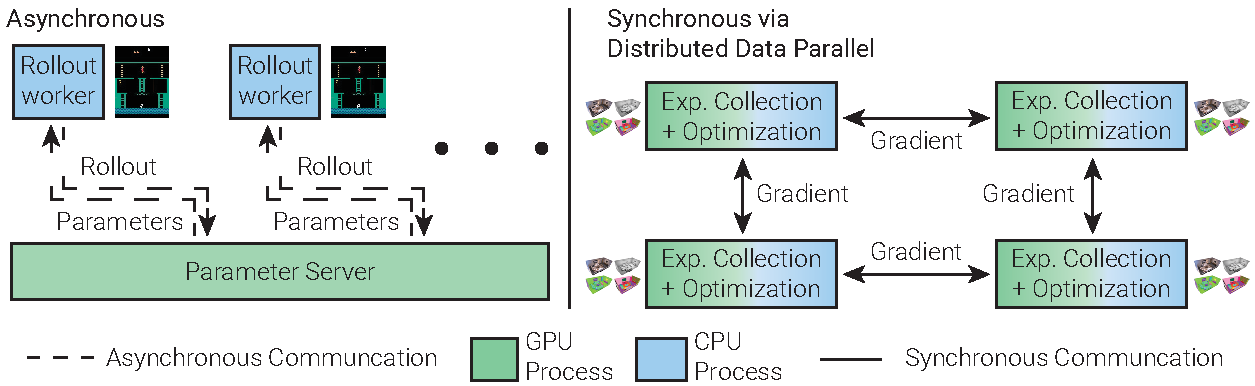
\includegraphics[width=\textwidth]{figures/related_work/ddppo}
    \caption{\textbf{Decentralized Distributed Proximal Policy Optimization (DD-PPO)}.
    This algorithm is included in the Habitat Lab as a baseline for training end-to-end visual navigation policies.
    It laid the foundation for the majority of the subsequent works in the field, and it is used in this thesis as well.
    While typical \acrshort{rl} have been trained in an asynchronous manner, DD-PPO uses a synchronous approach to train the agent in multiple environments at the same time.
    Figure from~\cite{wijmans2020}.}
    \label{fig:ddppo}
\end{figure}

Finally, there are different approaches that try to tackle the problem of rapidly adapting to unseen environments in visual navigation via meta-learning~\cite{wortsman2019, luo2021, zhang2022}.
These methods are trained on a variety of different environments (usually designated as tasks) and are able to generalize to unseen environments by learning a policy that can be quickly adapted to new environments.
And the recent progress in large language models (LLMs) has led to the possibility of using them to solve the visual navigation problem~\cite{Huang2023, Zhou2023} as well.
In this case, the LLMs are used as a reasoning module in charge of understanding the semantic information present on the environment.
They then share this information with different modules in charge of navigating to the specified goal.

\section{Sparsity and exploration methods}\label{sec:sparsity-and-exploration-methods}
To address the sparse reward and exploration problems, different approaches have been proposed.
Auxiliary tasks~\cite{jaderberg2016, ye2021} help the agent to explore the environment and gather extrinsic reward by maximizing pseudo-reward functions.
Curiosity-driven exploration~\cite{pathak2017} (depicted on figure \ref{fig:curiosity}) leverages on the error of the agent's ability to predict the next state to introduce a new intrinsic reward that enables the agent to explore the environment.
When dealing with procedurally-generated environments, a curriculum learning mechanism can be incorporated so the episodes are ordered by an exploration score~\cite{zha2020b}, and then the agent imitates the best ones.
This thesis also uses procedurally-generated environments, but it relies on a RL approach combined with reward shaping~\cite{ng1999, jestel2021} and $\epsilon\text{-}greedy$~\cite{mnih2013} techniques to learn to navigate in them.

\begin{figure}
    \centering
    \includegraphics[width=\textwidth]{figures/related_work/curiosity}
    \caption{\textbf{Curiosity-driven exploration} is a technique that uses the error of the agent's ability to predict the next state to introduce a new intrinsic reward that enables the agent to explore the environment.
    The agent learns a forward model that predicts the next state given the current state and action.
    The intrinsic reward is then computed as the error between the predicted and actual next state.
    Figure from~\cite{pathak2017}.}
    \label{fig:curiosity}
\end{figure}

\section{Simulation-to-reality transfer in robotic navigation}\label{sec:simulation-to-reality-transfer-in-robotic-navigation}
Deploying a model trained in simulation to a real robot is a challenging task.
Due to logistical constraints, training a model in the real world —especially with RL techniques— is often impractical, prompting the use of alternative methods to address this challenge.
For example,~\cite{kim2022} proposes a monocular vision-based time-to-collision estimation for small drones by domain adaptation of simulated images.
Their method converts simulated images into real-like synthetic images using a sim-to-real method.
This is done with the aim of minimizing efforts and time invested in the collection of training datasets within real-world scenarios, while simultaneously maximizing the advantages inherent in simulated environments.

Overall, it is necessary to develop methods that allow to efficiently transfer the knowledge learnt in simulation to the real world.
Different approaches have been proposed to solve this problem.
In ~\cite{kadian2020}, an exact replica of a real scenario is simulated (see figure~\ref{fig:sim2real}).
This allows the authors to explore the behavior of visual navigation policies both in simulation and in reality and how their performance correlates.
For instance, CAD2RL~\cite{sadeghiCAD2RLRealSingleImage2017} system achieved remarkable success in training a collision avoidance policy entirely within a simulated environment.
This breakthrough was subsequently tested on real aerial drones, with promising results.
By focusing on simulation refinement~\cite{Son2020}, the accuracy of simulations can be improved by exploiting the disparities between simulated and real-world observations.
In the field of locomotion, training legged robotic systems in a simulated environment and subsequently transferring the acquired policies to real-world applications~\cite{Hwangbo_2019, agarwal2022} has always been a challenging task.

\begin{figure}
    \includegraphics[width=\textwidth]{figures/related_work/sim2real}
    \caption{\textbf{Simulation-to-reality transfer} is a challenging task in robotic navigation.
    In this example, a real-world scenario is simulated to explore the behavior of visual navigation policies both in simulation and in reality.
    The authors use a simulated environment that closely resembles the real-world scenario, allowing them to train and evaluate their policies in a controlled setting.
    Figure from~\cite{kadian2020}.}
    \label{fig:sim2real}
\end{figure}

For the problem of \acrshort{vsn}, the study by~\cite{gervet2022} shows how different approaches behave in real-world settings.
They compare the performance of different \acrshort{vsn} methods in simulated and real-world environments, concluding that modular-learning approaches outperform end-to-end learning methods in real-world scenarios.
Interestingly, the conclusion of chapter~\ref{ch:ros4vsn:-enable-real-world-robotic-visual-semantic-navigation}, is the same as in~\cite{gervet2022}: that modular-learning approaches are the best ones for deployment in the real world.

\section{Offline Reinforcement Learning}\label{sec:offline-reinforcement-learning}

Offline reinforcement learning (offline RL) refers to learning a policy from a fixed dataset of environment interactions, without additional online exploration~\cite{levine2020} (figure \ref{fig:diagram-offline}).
This paradigm is appealing for robotics, where collecting data is costly or risky, since it allows agents to leverage large logs of prior experiments or demonstrations.
However, a core challenge in offline RL is distributional shift: the learned policy may choose state-action pairs not well-covered by the dataset, leading to arbitrarily bad value estimates and unstable policy updates.
Over the past years, a number of algorithmic strategies have been proposed to address this issue and enable effective offline learning of robotic skills.

\begin{figure}
    \includegraphics[width=\textwidth]{figures/related_work/diagram_offline}
    \caption{\textbf{Offline reinforcement learning} is a paradigm that allows training models using fixed datasets, without the need for online data collection.
    In this diagram, the offline RL process is depicted, where a dataset of environment interactions is used to train a policy.
    The policy is then evaluated in the environment, and the process is repeated until convergence.
    Figure from~\cite{levine2020}.}
    \label{fig:diagram-offline}
\end{figure}

\subsection{Conservative Value Estimation}\label{subsec:conservative-value-estimation}

One line of work imposes \textit{pessimism} in value function learning to avoid overestimating unseen actions.
For example, Conservative Q-Learning (CQL)~\cite{conservative} augments the Bellman objective with a penalty on Q-values for out-of-distribution actions.
By learning a deliberately conservative Q-function (lower-bounding the true values), CQL prevents the policy from exploiting spurious high rewards for actions outside the dataset support.
Similarly, Implicit Q-Learning (IQL)~\cite{kostrikov2022offline} avoids querying unseen actions altogether during training.
Instead of a max over actions, IQL uses an expectile regression to estimate the value of the \textit{best} in-dataset actions, then extracts a policy via advantage-weighted behavior cloning.

\subsection{Policy Constraints and Behavior Regularization}\label{subsec:policy-constraints-and-behavior-regularization}

Another broad strategy is to constrain the learned policy to stay close to the behavior policy that generated the data.
A prominent example is Batch-Constrained deep Q-learning (BCQ)~\cite{Fujimoto2018OffPolicyDR}, which modifies the Q-learning update to consider only actions that are likely under the offline dataset instead of maximizing over all actions.
In practice, BCQ trains a generative model (e.g. a VAE) to produce candidate actions similar to those in the dataset, ensuring that the policy cannot stray far from logged behavior.
Likewise, Bootstrapping Error Accumulation Reduction (BEAR)~\cite{Kumar2019StabilizingOQ} and Behavior-Regularized Actor-Critic (BRAC)~\cite{Wu2019BehaviorRO} add explicit divergence penalties (e.g. KL or MMD) to keep the learned policy distribution close to the dataset behavior policy.
By limiting policy deviation, these methods address bootstrapping error and distribution shift, effectively preventing the agent from choosing out-of-distribution actions with erroneously high value estimates.
Variants of this idea combine RL updates with imitation learning: for instance, Advantage-Weighted Actor-Critic (AWAC)~\cite{Nair2020AcceleratingOR} and Critic-regularized Regression (CRR)~\cite{NEURIPS2020_588cb956} constrain the policy toward the dataset behavior while weighting actions by their estimated advantages, thus improving performance without sacrificing stability.
Overall, policy constraint and behavior regularization approaches have proven effective both in simulation and in real-world settings by leveraging the data’s demonstrated behaviors as an anchor.

\section{Meta Reinforcement Learning}\label{sec:meta-reinforcement-learning}

\section{RL For Navigation}\label{sec:navigation}

\subsection{Problem Formulation}\label{subsec:problem-formulation}

We address the VSN problem by using Reinforcement Learning (RL).
Thus, navigation can be described as a partially observable Markov decision process (POMDP), in which the agent, \ie, a robot, navigates through an environment and tries to reach a determined object.
This problem is known in the literature as the ObjectNav task~\cite{batra2020}.

Formally, given an initial observation distribution $p_0$, for the step $t$ the agent receives an observation $o_t \sim p_0(o)$ based on state $s_t$, which in our case is just an RGB image of what the robot observes.
The agent takes action $a_t$, obtains reward $r_t$ from the environment and receives a new observation $o_{t+1} = \mathcal{T} (o_{t+1}|o_t, a_t)$, where $\mathcal{T}$ is the transition function.
An episode is a sequence of $\left(o_t, a_t, r_t\right)$ tuples that form a trajectory.
The episode ends when the agent reaches the goal or the maximum number of steps ($H$).
An episode is considered a success if the agent reaches the goal within the step horizon $H$.

The goal is to find an optimal policy $\pi^*$ that maximizes the cumulative reward over an episode.
This policy maps observations to a probability distribution over actions that is specified as follows,
\begin{equation}
    \label{eq:op_policy}
    \pi^*=\argmax\limits_\pi\mathbb{E}_{\mathcal{T}\sim\pi}[R_H],
\end{equation}
where $R_H=\sum_{t=1}^H \gamma^{t-1}r_t$ is the return, \ie the cumulative reward over an episode, and $\gamma$ is a discount factor.
In navigation tasks, neural networks with parameters $\theta$ are often used to parameterize the policy $\pi_\theta$.

\subsection{Visual Semantic Navigation}\label{subsec:visual-semantic-navigation}

Learning to navigate in a given environment is a challenging task.
First, the reward signal coming from the environment is usually sparse~\cite{sutton2018, pathak2017}.
These sparse rewards lead to a quite difficult training process.
%Second, the agent has to balance an exploration of the environment to obtain experience and the exploitation of the previous experience in order to obtain successful episodes~\cite{sutton2018, mnih2013}.
Second, we need to find a balance between the exploration and exploitation of the environment to achieve successful experiences that drive the agent's learning process~\cite{sutton2018, mnih2013}.
Finally, the agent architecture has a direct impact on how it learns.
State-of-the-art approaches use a feature extractor followed by recurrent units to process temporal information coming from the images.
%For navigation tasks, a common agent architecture consists of a CNN feature extractor and an RNN that outputs the action distribution.

\textbf{Sparse rewards and long horizon.}
%In visual navigation, sparse rewards are a common issue due to the nature of the task, \ie reaching a specific target in an environment.
Sparse rewards are a common issue due to the nature of the navigation tasks, \ie reaching a specific target in an environment.
The most straightforward way to define a reward in navigation problems is to let the environment provide a fixed amount when the agent reaches the goal.
This means the agent has to face an environment in which:
1) in the best case, most of the reward signal is zero except for the step in which the agent reaches the goal and obtains a certain amount of reward;
and 2) if the agent does not reach the target it does not receive any reward.
This situation worsens with large temporal horizons, because the more steps, the higher the sparsity of the reward is.

To mitigate the sparse reward problem, we use a technique called reward shaping.
It consists in modifying the original reward signal via incorporating domain knowledge.
For navigation, we leverage on the \textit{distance reward}~\cite{wijmans2020}, defined as:
\begin{equation}
    \label{eq:rew_shaping}
    r_t = -d(s_t, target) + d(s_{t+1}, target) - r_s + r_T,
\end{equation}
where $d(s_t, target)$ computes the geodesic distance between agent's position at state $s_t$ and $target$'s position.
$r_T$ is the \textit{terminal reward}, a fixed amount given only when the agent reaches the target and $r_s=0.01$ is the \textit{slack reward}, also a fixed amount that penalizes each step.
The goal of the \textit{distance reward} function is to give a constant reward signal to the agent that increases as the agent approaches the target.
In section~\ref{subsec:miniworld-maze-results} we compare the \textit{distance reward} against what is usually referred to as the \textit{navigation reward}, which consists only of the slack reward and the terminal reward $r_t = -r_s + r_T$.

\textbf{Exploration vs. Exploitation.}
%As we have mentioned, in a navigation problem, our agent must explore the environment in order to find the trajectories that return the maximum amount of reward without surpassing the temporal horizon of $H$ steps.
%This exploration has to be balanced with respect to the exploitation process, in which the agent uses the previous knowledge to actively select the best actions to obtain the shortest successful episodes.
As we have mentioned, the exploration process has to be managed to encourage the agent to choose actions that it would not otherwise select.
To address this issue, we leverage the technique known as $\epsilon\text{-}greedy$~\cite{mnih2013}.
This solution \emph{controls} the action that is being selected by the agent, usually during the learning process.
Given an $\epsilon \in [0, 1]$, an action $a_t$ is selected as
\begin{equation}
    \label{eq:eps-greedy}
    a_t = \begin{cases}
              \argmax\pi_\theta & \mbox{with probability 1-$\epsilon$,}     \\
              rand(a) \in \mathcal{A} & \mbox{with probability $\epsilon$,} \\
    \end{cases}
\end{equation}
where $\mathcal{A}$ defines the action space.
Typically, $\epsilon$ starts at $1$ and it decays with the iterations.
In the beginning of the learning process, \ie when $\epsilon$ is high, random actions are sampled more often, encouraging the agent to explore the environment.
As the training process advances, lower $\epsilon$ values permit the agent to exploit the model knowledge to select the best action.
This introduces a balance between exploration and exploitation.

\textbf{Agent architecture.} We encode the agent as a parameterized model consisting in a CLIP~\cite{khandelwal2022} visual encoder connected to two actor-critic LSTMs that output a discrete distribution over the action space and the value, respectively.
A diagram of the implemented agent can be found in figure~\ref{fig:network_clip_diagram}.
To train the models, we use Proximal Policy Optimization (PPO)~\cite{schulman2017}, an on-policy RL algorithm.

\begin{figure}[t]
    \centering
    \includegraphics[width=0.8\linewidth]{figures/understanding_vsn/network_clip_diagram}
    \caption{\textbf{Model diagram}. This figure contains a high level representation of the model used: a visual encoder followed by an actor-critic module encoded by LSTMs. The visual encoder is frozen and we only train the actor-critic module.}
    \label{fig:network_clip_diagram}
\end{figure}


\subsection{Experiments}

\begin{table}[t]
    \centering
    \begin{tabular}{c|cccc}
        \toprule
        \textit{\textbf{Setup}} & \textit{\textbf{SR (\uparrow)}} & \textit{SPL (\uparrow)} & \textit{\textbf{Distance to Goal (\downarrow)}} \\ \midrule
        1                       & 5/15                            & 33,33\%                 & 49                                              \\
        2                       & 5/15                            & 33,33\%                 & 91                                              \\
        3                       & 5/15                            & 33,33\%                 & 70                                              \\
        4                       & 3/15                            & 20,00\%                 & 97                                              \\
        5                       & 1/15                            & 6,67\%                  & 61                                              \\
    \end{tabular}
    \caption{Evaluation of MetaNav on the VSN task. Results obtained with continuos evaluation}
    \label{tab:pirlnav}
\end{table}


\begin{table}[t]
    \centering
    \begin{tabular}{c|cccc}
        \toprule
        \textit{\textbf{Setup}} & \textit{\textbf{SR (\uparrow)}} & \textit{SPL (\uparrow)} & \textit{\textbf{Distance to Goal (\downarrow)}} \\ \midrule
        1                       & 0.80                           & 38\%                 & 49                                              \\
        2                       & 0.61                            & 27\%                 & 91                                              \\
        3                       & 0.55                          & 26\%                 & 70                                              \\
        4                       & 0.16                            & 5\%                 & 12                                              \\
        5                       & 0.25                            & \%                  & 61                                              \\
    \end{tabular}
    \caption{Evaluation of MetaNav on the VSN task. Results obtained with per episode evaluation}
    \label{tab:pirlnav}
\end{table}


\chapter{Conclusions}\label{ch:conclusions}

\lettrine{\textcolor{accent_color}{T}}{his} thesis has focused on the exploration of robotic visual navigation, specifically in the context of visual semantic navigation, and how it can be improved through the use of reinforcement learning methodologies.
The main objective has been to develop a new ROS~\cite{ros} framework that allows the integration of different algorithms and environments, as well as to explore new approaches to offline reinforcement learning and meta imitation learning for robotic visual navigation.
Concretely, the thesis has focused into solving \acrshort{objnav}


\section{Contributions}\label{sec:contributions}
\begin{itemize}
    \item \textbf{ROS4\acrshort{vsn}:} A new framework for robotic visual navigation that allows the integration of different algorithms and environments.
    \item \textbf{Offline Reinforcement Learning for Robotic Visual Navigation:} A new approach to offline reinforcement learning for robotic visual navigation that uses a combination of imitation learning and reinforcement learning.
    \item \textbf{Meta Imitation Learning for Robotic Visual Navigation:} A new approach to meta imitation learning for robotic visual navigation that uses a combination of meta-learning and imitation learning.
\end{itemize}


\section{Discussion and Further Improvements}\label{sec:discussion-and-further-improvements}


\section{Future Research Lines}\label{sec:future-work}


\section{Scientific Contributions}\label{sec:final-remarks}

During the development of this thesis, it has been possible to contribute to topics of this thesis in several ways.
It has also been possible to contribute to other topics that, although not directly related to the thesis, have been developed in parallel.
These have come from side projects or collaborations with other research groups and have contributed to the development of this thesis.
All of them are summarized in the following subsections.

\subsection{Contributions directly related to the thesis}\label{subsec:contributions-directly-related-to-the-thesis}

\begin{itemize}
    \item \cvpub{\textbf{Gutiérrez-Alvarez C.}, Ríos-Navarro P., Flor-Rodríguez-Rabadán R., Acevedo-Rodríguez F.J., López-Sastre R.J., \textit{Visual Semantic Navigation with Real Robots}, in Applied Intelligence, 2024.}
    \item \textbf{Gutiérrez-Alvarez C.}, Acevedo-Rodríguez F.J., López-Sastre R.J., Kanezaki A., OffNav: \textit{Offline Reinforcement Learning for Visual Semantic Navigation}, in ICRA Human-aligned Reinforcement Learning for Autonomous Agents and Robots Workshop, 2024.
    \item \textbf{Gutiérrez-Alvarez C.}, Ríos-Navarro P., Flor-Rodríguez-Rabadán R., Acevedo-Rodríguez F.J., López-Sastre R.J., \textit{Evaluation of Visual Semantic Navigation Models in Real Robots}, in IROS Late Breaking Results, 2023.
    \item \textbf{Gutiérrez-Alvarez C.}, Hernández García S, Nasri N, Cuesta-Infante Alfredo, López-Sastre RJ, \textit{Towards Clear Evaluation of Robotic Visual Semantic Navigation}, in ICARA, 2023.
    \item \textit{Participation in the project \textbf{NAVIGATOR-D} (PID2023-148310OB-I00)}, funded by the Spanish Ministry of Science and Innovation.
    \item \textit{Participation in the project \textbf{AIRPLANE} (PID2019-104323RB-C31)}, funded by the Spanish Ministry of Science and Innovation.
\end{itemize}

\subsection{Side contributions}\label{subsec:side-contributions}

\begin{itemize}
    \item Flor-Rodríguez-Rabadán R., \textbf{Gutiérrez-Álvarez C.}, Acevedo-Rodríguez F.J., Lafuente-Arroyo S., López-Sastre R.J., \textit{SEMNAV: A Semantic Segmentation-Driven Approach to Visual Semantic Navigation}, in ArXiv, 2025.
    \item Nasri N, \textbf{Gutiérrez-Álvarez C.}, López-Sastre RJ, Lafuente-Arroyo S., Maldonado-Bascón S. \textit{Realistic Continual Learning Approach using Pre-trained Models}, in ArXiv 2024.
    \item Blanco-Fernández E., \textbf{Gutiérrez-Alvarez C.}, Nasri N., Maldonado-Bascón S., López-Sastre R.J., \textit{Live Video Captioning}, in Multimedia Tools and Applications, 2025.
    \item Lafuente-Arroyo S., Maldonado-Bascón S., Delgado-Mena D., \textbf{Gutiérrez-Alvarez C.}, Acevedo-Rodríguez F.J., \textit{Multisensory Integration for Topological Indoor Localization of Mobile Robots in Complex Symmetrical Environments}, in Expert Systems with Applications, 2023.
    \item Nasri N, López-Sastre RJ, Pacheco-da-Costa S, Fernández-Munilla I, \textbf{Gutiérrez-Álvarez C.}, Pousada-García T, Acevedo-Rodríguez FJ, Maldonado-Bascón S. \textit{Assistive Robot with an AI-Based Application for the Reinforcement of Activities of Daily Living: Technical Validation with Users Affected by Neurodevelopmental Disorders}, in Applied Sciences, 2022.
\end{itemize}

% \section*{Acknowledgment}
% This research was funded by project AIRPLANE, with reference PID2019-104323RB-C31, from the Ministry of Science and Innovation of Spain.

\bibliographystyle{IEEEtran}
\bibliography{library}

\end{document}
